%% LaTeX2e class for student theses
%% sections/apendix.tex
%% 
%% Karlsruhe Institute of Technology
%% Institute for Program Structures and Data Organization
%% Chair for Software Design and Quality (SDQ)
%%
%% Dr.-Ing. Erik Burger
%% burger@kit.edu
%%
%% Version 1.2, 2016-09-20


\iflanguage{english}
{\chapter{Appendix}}    % english style
{\chapter{Anhang}}      % german style
\label{chap:appendix}


%% -------------------
%% | Example content |
%% -------------------
\section{Calculation of Bit Error Ratio}
\label{sec:appendix:calcBER}	
\setcounter{figure}{0}
		
In order to analyze the performance of the optical link developed in this thesis, the theoretical framework of the Gaussian channel in information theory, as shown in \ref{fig:gaussianchannel}, is used as a reference. The channel is a time discrete channel that outputs through $Y_i$, at time $i$, the sum of input $X_i$ and noise $Z_i$ \cite{ThomasInfoTheory91}. The noise profile has a Gaussian distribution, and has a variance $N$. Since energy is the biggest constraint in most communication systems. Assuming a power level of $\sqrt{P}$ and noise variance $N$ for the high level of one bit. The probability of error is $P_e = 1 - \erfc{\sqrt{\frac{P}{N}}}$, where the complementary error function is defined as:

\begin{align}
\erfc{(z)}=\frac{2}{\sqrt{\pi}} \int_z^{\infty} e^{-t^2}dt
\end{align}

This effectively converts the Gaussian channel into a discrete binary symmetric channel with crossover probability $P_e$ \cite{ThomasInfoTheory91}. This allows for a quantization of the channel and be able to perform error correction on the data transmitted.

\begin{figure}[!ht]
  \includestandalone[width=0.3\textwidth]{tikz/gaussianchannel}
  \centering
  \caption{The Gaussian channel. Adapted from \cite{ThomasInfoTheory91}.}
  \label{fig:gaussianchannel}
\end{figure}

The bit error probability is calculated as:

\begin{align}
\text{BER} = p(1r)\int_{-\infty}^{u_s} w_1(u)du + p(0r)\int_{u_s}^{\infty} w_0 (u)du
\end{align}

where the optimum decision threshold $u_s$ is used as the limit between a 0 and a 1 being correctly (and incorrectly) detected, considering a Gaussian probability density function (PDF), and assuming that electronic noise dominates and nearly equivalent probabilities of a 1 and a 0 value is received, the minimum bit error probability can be reduced to:

\begin{align}
\text{BER} &  = \frac{1}{2} \erfc \left( \frac{\sqrt{\gamma}}{\sqrt{2}} \right)
	 	  	= \frac{1}{2} \erfc \left( \frac{\sqrt{\text{SNR}}}{\sqrt{2}} \right)
\end{align}

This calculation applies to return-to-zero bit patterns with a 50\%, and the bit error parameter $Q$ is equated to the square root of the signal-to-noise ratio (SNR). Other modulation formats have different weighs for the error function but this provides a good rule-of-thumb of the expected bit error probability.

%% ---------------------
%% | / Example content |
%% ---------------------

\section{Gate Voltage Theory and Implementation}
\label{sec:appendix:gatevolt}

As pointed out in the work of Alloati \cite{gateAlloatti12}, electron and hole concentration in a semiconductor can be controlled by using external electric field. The model used is the metal-insulator-semiconductor (MIS). Assuming flat-band condition, no surface changes in the insulator and homogeneous, non-degenerate semiconductors, leading to the Fermi-Dirac distribution function and the further simplified Maxwell-Boltzmann exponential distributions.

Given n-type semiconductors, a positive voltage ($V_\text{gate}>0$) causes negative charge (due to being n-type, these are the majority carriers) \emph{accumulation}. If a negative voltage is applied ($V_\text{gate}<0$) the majority carriers are depleted. If the applied voltage is negative enough, the minority and majority carrier density is nearly equal and the charge is inverted. 

The potential energy $q\phi$ provides an indication of the band bending direction (i.e. positive potential energy bends the bands downwards, and viceversa). The corresponding Poisson equation is given by:

\begin{align}
\frac{\partial^2 \phi}{\partial x^2} = \frac{2 k_B T N_{e,0}}{\epsilon_s} 
\left[ \left( e^{q\phi /k_B T} - \frac{q\phi}{k_B T} - 1 \right) +
\frac{N_{h,0}}{N_{e,0}}  \left( e^{q\phi /k_B T} + \frac{q\phi}{k_B T} - 1 \right) 
\right]
\end{align}

Where $N_{h/e,0}$ is the initial concentration of holes or electrons, respectively. If the insulator thickness $d$ is larger than the space-charge region, the electric field in the insulator and semiconductor reduces to:

\begin{align}
E_xi(x=0^-) = \frac{V_\text{gate}}{d}; E_xs(x=0^+) = \frac{\epsilon_i}{\epsilon_s} \frac{V_\text{gate}}{d}
\end{align}

In order to implement the external gate voltage, highly-mobility electron accumulation layer is induced in the semiconductor interface. %The breakdown voltage in \ce{SiO2} is \SI{1}{\volt /\nano\meter} 

%\section{Afterword}

%Afterwords are not a common trait in master thesis. I have not encountered one among the ones I have read through in the initial phase of my master thesis, and probably it is meant for longer, more fruitful thesis projects, such as a doctor degree. Nonetheless, and provided someone is going to go as far as this page to read my work in the past months, I felt it is important for me to share my experience through the lens of my skewed perception in life.

%In 2012, I went to a festival in London, England, and there were some booklets that featured some quotes, one which has resonated in my brain for that long: \emph{Do not fear mistakes; there are none.} This quote is, allegedly by Miles Davis, a famed jazz trumpetist of whom I bought my first jazz album, back in 2010, named ``Kind of blue''. I dug further deep to try and find if the quote was accurate, and ended up reading a paper called ``\emph{Out of notes:} Signification, Interpretation and the Problem of Miles Davis'' by Robert Walser. While unimportant for the time being here, the paper goes on about to develop on the null theorem that Davis was, above all, a flawed musician and trumpetist, albeit a very creative one. I had to go through several records of other trumpeters to unveil this realization. Everything Davis recorded sounds \emph{off}, to some extent. A sense of disconnection, or maybe lack of commitment to creating the pieces. 

%With this in mind, I would like to point out a severe flaw of mine: I believe in making mistakes. I have gotten so far in life by making mistakes, learning from them, and move on, not making them again (or at least, not consciously). That has been my path through life, through jobs, and more recently, through a second academic endeavor in an area I had no previous knowledge of (optics) but that I deeply enjoyed and wanted to know more about. Unfortunately for me, the lenience (or lack thereof) of a system I deeply disagree with, along with personality traits that may seem more defiant than indulgent, lead me to making a flurry of mistakes that, to this day, haunted every single morning I wanted to say ``don't worry, learn, move on, don't make it again''. It felt always more as a cross to carry. The mistake was an anchor towards inaction. With few days before finally finishing the project and moving on with my life, these past six months lead me to understand that science is not for me, and I should focus on my career.

%Melancholy aside, I would like to point out some things I learned during the process that could be potentially of help to someone in the future, and to remind those who fail, that there really are no mistakes. 

%First and foremost, always set a communication path with your supervisor that works both ways. I personally do not like calling or talking to people because it makes me anxious, so I try to keep communications to text, and if possible, only to institutional means, because I believe in the privacy bubble that separates work and your personal life. I do not like to contact work people through their personal phone because I find it intrusive, but sometimes it is necessary to do so, especially if there are no significantly better institutional tools.

%Laser pre-characterization was an incredibly arduous task for me, since I had never used the tools beforehand. If you feel like you need some practice with dummy devices, ask for them. For some reason, the concept of ``dummy'' varies greatly from person to person. In my perspective, a dummy chip is a device that no longer works properly but is useful to scratch, to break, toy around and understand the principle in which a device works. As I mentioned, I feel very anxious when I am given the working version of anything and with a huge sign that says ``this thing is incredibly valuable and there is one existing copy in the whole planet, be extremely careful or your whole career will be ruined along with this device''. This was not how I was told this, but I did not feel safe having the working part that ended up in the first module. I scratched it heavily, and I was not 100\% sure that the device was properly tested. I did not understand the mechanics, the procedure, or the aim of the measurement. This lead to several mistakes down the road: Improper manipulation of other HCSELs; spending a whole day trying to get power out of a working HCSEL with poor contacting; A bad measurement of the optical spectrum of a HCSEL array, among others. 

\section{Schematic Diagram of IME05-MS3 Full Transmitter}

The full optical transmitter is represented in figure \ref{fig:fulltx}. The light source (HCSEL) is shown at the left side of the figure. At the center, the SOH is shown, with an schematic representation of the different optical paths available on-chip: 
\begin{itemize}
\item Channels 1-4 are single-channels, with input from the HCSEL via inverted taper or the GC. An MMI (not shown) inverts the inputs at the output, which can be at the GC or a SMF via taper.
\item Channels 5-8 are combined channels, with the following options:
	\begin{itemize}
		\item One output per channel to a SMF via taper
		\item Channels 5 and 6 combined through MMI to output 9
		\item Channels 7 and 8 combined through MMI to output 8
		\item Channels 5,6,7 and 8 combined through MMI to output 0 (via taper or grating coupler)
	\end{itemize}
\end{itemize}

\begin{figure}[!ht]
\centering
  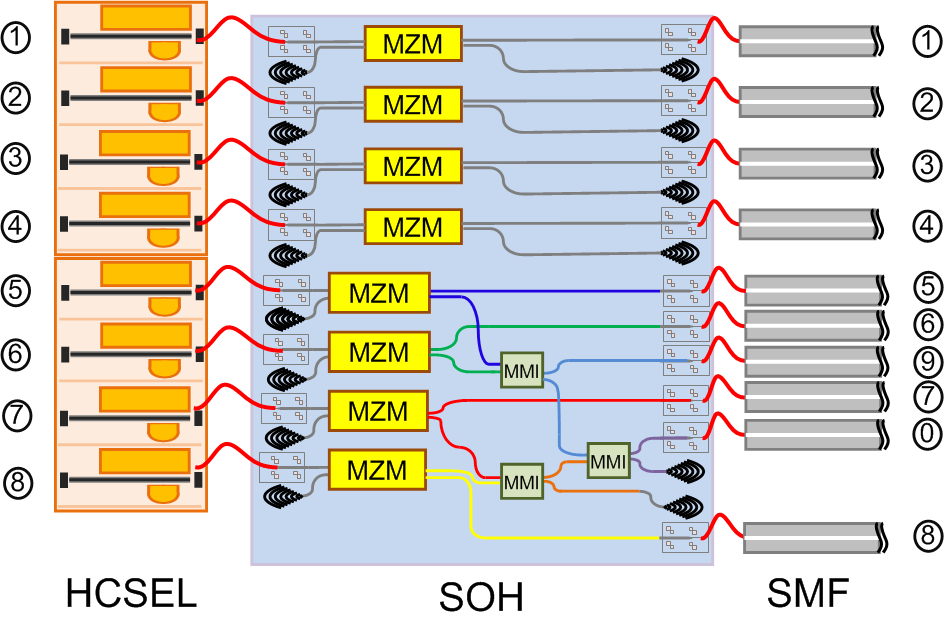
\includegraphics[width=0.9\textwidth]{visio/Schematic}
  \caption{Schematic diagram of full transmitter. A HCSEL array of 8 devices is connected via PWB to an SOH MZM chip. Coupling of light can also be done through grating couplers. 4 MZM channels can be independently measured, and 4 additional MZM channels can be combined for WDM or PSM transmission.}
  \label{fig:fulltx}
\end{figure}

%\section{Local Deposition}

\section{Device Manufacturing: Local Deposition}
\label{ch:LD}
Organic materials are processed in a different manner than inorganic materials. While inorganic materials have to be processed, for the most part, by means such as physical vapor deposition, cathodic arc deposition or electrospray deposition, to name a few, organic materials have the advantage of being not only deposed but also printed. In the present work, an automated method for local material deposition is implemented. 

%\subsection{Current State}

Local deposition means that a polymer dissolved in a liquid is passed through a slit or a slot, which is filled with the electro-optical chromophore, and then developed for further processing. For the local deposition of materials, a set of stepper motors with fine steps are utilized and driven with a \textbf{ESP300 Motion Controller/Driver} manufactured by Newport, which allows for 3-axis movement and positioning of devices.  %A right-hand cartesian coordinate system is chosen, such that the chip is visualized with a camera, and the movement corresponds to the spatial shift observed through the camera (i.e. if the motor system is "reversed" then movements are mirrored in software).  \par\medskip

%The most important offsets and distances indicated in figure \ref{fig:chiplo} are the following:
%\begin{itemize}
%	\item $\mathbf{d_n}$, which is the length of a specific device that needs to be processed. This has been set as a variable since a single chip may contain different device lengths, but is not common to have different lengths along the $y$-axis.
%	\item  $\mathbf{d_n/2}$ is the middle point of a device, and this is the region where the droplet is prepared as it is far from the optical devices but has a relatively equal surface height to avoid changes in the droplet size.
%	\begin{itemize}
%		\item In some cases, a position $\mathbf{x^*_n}$ can be used in case a specific overlap with a sensitive optical device occurs at the middle of the device. Further, this will be the offset of choice to describe the positioning as it is the most generalized position. 
%	\end{itemize}
%	\item $\mathbf{y_q}$ is the distance in the $y$-axis in which the droplet is prepared for deposition, and $\mathbf{y_p}$ is the device pitch (i.e. distance between two devices).   
%\end{itemize}
%
%\begin{figure}[!ht]
%\centering
%  \includestandalone[width=0.8\textwidth]{tikz/chiplo}
%  \caption{Chip layout for local deposition. (0,0) indicates the chip origin.}
%  \label{fig:chiplo}
%\end{figure}

%Figure \ref{fig:zaxislo} shows the layout of the vertical axis, in which the chip surface, at position $z_0$, is going to be subject to local deposition using a biomedical grade needle. The needle is previously wetted with the polymer solution of interest and the chip is allocated in the chip mount. By using a camera, the height $z_v$ is the height at which the needle is visible through the camera. The needle is positioned at $(x^*_n, q_n,z_v)$. The needle is approximated to the surface $z_0$ using steps $\Delta z$ in order to avoid direct contact with the optical layout (as the needle can easily bend and break, or damage the optical devices). The position can be detected by direct visualization. Once the needle is at exactly $z_0$, the needle is slowly lifted to $z_m$ to form the meniscus\footnote{in the figure, the shape utilized to picture the meniscus is a gaussian, as this proved to be the the fastest solution to show the meniscus on both sides exploiting the layering capabilities of TiKz. This, however, is not an accurate representation of the physical phenomenon due to surface tension which has a form closer to a cosine. For schematic purposes, though, the meniscus is adequately represented by the gaussian used in the figure.} which will depose the polymer into the slot. The needle is then moved along the $x$-axis along the device to deposit the material into the slot twice, and the needle is lifted to position $z_v$. The organic polymer should be deposited only in the slot since it can produce undesired effects after the electrical packaging.

%A semi-automatic mode is implemented to approach the needle to the surface. There is no collision warning or lock-out conditions for the basic implementation. 

%\begin{figure}[!ht]
%\centering
%  \includestandalone[width=0.7\textwidth]{tikz/zaxislo}
%  \caption{$z$-axis layout for local deposition.}
%  \label{fig:zaxislo}
%\end{figure}

%\subsection{Local Deposition Method}

%\subsection{Process Flow}

%The main process flow is detailed in figure \ref{fig:ldbd}. 

%\begin{figure}[!ht]
%\centering
%  \includestandalone[width=0.7\textwidth]{tikz/ldbd}
%  \caption{Local deposition block diagram.}
%  \label{fig:ldbd}
%\end{figure}

%\subsection{Software Requirements}

%\clearpage
%\newpage
%% Schematic representation of mach zender interferometer
% Modified from a version created by Henrik Kröger, https://github.com/derhedwig/fiberoptics/blob/master/auswertung.tex
% Author: Orlando Torres (2016)

\documentclass[12pt,a4paper,preview]{standalone}
\usepackage{amsmath} % Required for \varPsi below
\usepackage{tikz,pgfplots}
\usetikzlibrary{calc}
\usetikzlibrary{patterns}
\usetikzlibrary{backgrounds}
\usepackage{caption}
\usepackage{booktabs}
\usepackage{multirow}
\usepackage{siunitx}
\usepackage{rotating}
\usepackage{pdflscape}
\usepackage{array} 
\usepackage{graphicx}
%\sisetup{binary-units = true,table-format=7.0}

\begin{document}

\begin{landscape}
%\minipage{1.08\textwidth}
%\addtolength{\tabcolsep}{-1.0pt}
\begin{table}[htbp]
\centering
\newcommand*{\tpb}[1]{{\parbox[c]{10cm}{\raggedright #1}}}%
\newcommand*{\tpd}[1]{{\parbox[c]{4cm}{\raggedright #1}}}%
\scalebox{0.9}{
\begin{tabular}{@{}lllll@{}}
\toprule
ID & Feature                          & Description                                                                                                                                                                      & Priority & Status \\ \midrule
1  & \tpd{Automatic Dispensing }            & \tpb{The dispense mechanism for polymers is mostly automated. }                                                                                                                        & Top      & Open   \\\midrule
2  & \tpd{Double Slot Deposition }          & \tpb{Dispense mechanism can deposit a polymer on a double slot simultaneously  }                                                                                                       & High     & Open   \\\midrule
3  & \tpd{Column Deposition }               & \tpb{Dispense mechanism can deposit a polymer on a double slot simultaneously in an column of equally-sized devices        }                                                           & High     & Open   \\\midrule
4  & \tpd{Multi-column Deposition }         & \tpb{Dispense mechanism can deposit a polymer on a double slot simultaneously in multiple columns of equally-sized devices  }                                                          & High     & Open   \\\midrule
5  & \tpd{$z$-axis tolerancing }            & \tpb{Take into account leveling differences of the chip due to manufacturing tolerances to avoid device damage or needle breakage.   }                                                 & Low      & Open   \\\midrule
6  & \tpd{$xy$-axis tolerancing}            & \tpb{Take into account $xy$-plane alignment of the device for roll, pitch and yaw (rotations in $x$-, $y$- and $z$-axis, respectively) }                                               & Medium   & Open   \\\midrule
7  & \tpd{Multiple Polymer Dispensing }     & \tpb{Enable the user to dispense multiple types of polymer at specific columns or row sets.}                                                                                           & Low      & Open   \\\midrule
8  & \tpd{Matrix Deposition}                & \tpb{Dispense mechanism can have different column, row, and device settings in the advanced menu.} 																			& Low      & Open   \\\midrule
9  & \tpd{Height Detection  }               & \tpb{Use PID controller feedback in the motor driver to detect collision.}                                                                                                             & Low      & Open   \\\midrule
10 & \tpd{Report Generation}                & \tpb{Generate report of activities with time stamps, total duration of deposition, location of polymers, device sizes, offsets, and general calculations and detections.}              & Medium   & Open   \\\midrule
11 & \tpd{Camera Visualization  }           & \tpb{Visualize the current layout using one of the cameras directly connected to the driving computer.  }                                                                              & Medium   & Open   \\\midrule
12 & \tpd{Full Field-of-View Visualization} & \tpb{Use a network arrangement to be able to observe both cameras at the same time using a single screen.   }                                                                          & Low      & Open   \\\midrule
13 & \tpd{Image Processing}                 & \tpb{Automated detection of offsets, locations, distances and devices.               }                                                                                                 & Low      & Open   \\ \bottomrule
\end{tabular}
}
\caption{Software requirements decision matrix.}
\label{table:softreqs}
\end{table}
\end{landscape}
%\end{sidewaystable}

\end{document}
%\clearpage
%\newpage

%\subsection{Security Requirements}

%The software developed should cover security features, implemented in order to avoid the damaging a chip. 

%The security requirements are detailed in the following list:

%\begin{itemize}
%\item \textbf{Collision warning:} Warns the user about a possible collision due to the following causes:
%	\begin{itemize}
%	\item The chip is moved towards the needle positioned to close to $z_0$ in the $xy$-plane (reference $z$-plane), meaning the needle could potentially move the chip from its position or break.
%	\item The chip is moved towards the needle positioned to close to $z_0$ in the $z$-plane (reference $z$-plane), meaning the needle could potentially bend and break due to excessive force applied and damage the chip.
%	\end{itemize}
%\item \textbf{Lock-out Condition:} This condition stops the machine at any condition that could potentially damage the chip without user interaction, such as reaching boundary positions or critical damage locations.
%%\end{itemize}

%\subsection{ESP300 Motion Controller/Driver}

%For the implementation of ESP300 functions, a few were not included due to the following reasons:

%\begin{itemize}
%\item \textbf{DIO Bit interactions:} Such as enabling or disabling motion, notifications, motion status, jog direction, etc. Are %not implemented because the direct control of GPIB is outside the scope of this experimental work and there is no specific request to have an external controller (other than the one provided in the motion controller itself) for this specific device.
%\item \textbf{Synchronized movement:} The ESP300 controller showed several problems when trying to move two axes (or three) at the same time. This reduces slightly the 
%\end{itemize}

\subsection{Graphic User Interface Improvements}

The local deposition software was refreshed to address the following issues:

\begin{itemize}
\item Constant software shutdown
\item Improved control schemes
\item Faster positioning
\end{itemize}

\begin{figure}[!ht]
\centering
\begin{tabular}{cc}
\subfloat[Top GUI]{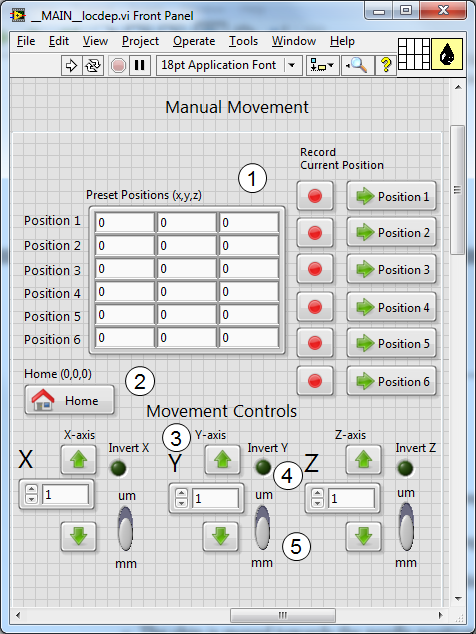
\includegraphics[width=0.4\textwidth]{figs/LOCDEP_top}\label{LDtop}} &
\subfloat[Bottom GUI]{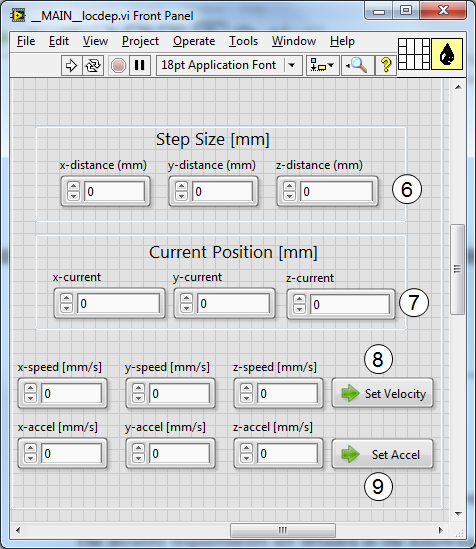
\includegraphics[width=0.4\textwidth]{figs/LOCDEP_bot}\label{LDbot}} \\
%\subfloat[]{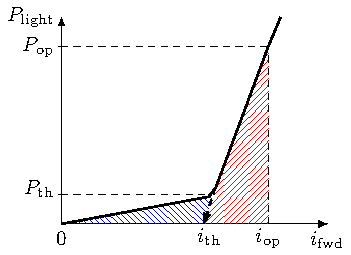
\includegraphics[width=0.4\textwidth]{tikz/LIcurve}} &
%\subfloat[]{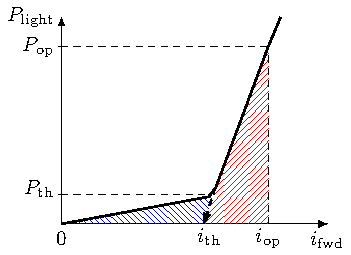
\includegraphics[width=0.4\textwidth]{tikz/LIcurve}} 
\end{tabular}
\caption{Local deposition GUI.}
\label{fig:locdep}
\end{figure}

The components of the GUI are the following:

\begin{enumerate}
\item \textbf{Preset positions}: Allows the user to record specific positions in the chip field which are commonly used to allow for faster navigation in the chip. The red button is used to record the current position, and the green arrow goes to the specific position. 
\item \textbf{Home}: Goes to the ``Home'' position at (0,0,0). The flow always starts by moving the $z$-axis before moving the $x$ and $y$ axes, for security purposes.
\item \textbf{Movement controls}: The arrows move in the positive direction with respect to the home position (0,0,0). This means that, when the button going up is pressed, the motors will move in the positive direction, the number of units in the number field between the two arrows. 
\item \textbf{Invert movement}: This button, when enabled (light is ``ON''), will move in the opposite direction. This was implemented since the $z$-axis considers moving in the positive direction as ``moving down'', which can be confusing for some users.
\item \textbf{Magnitude switch}: This changes the units of movement from millimeters to micrometers depending on the position of the rocker. 
\item \textbf{Step size}: Shows the step size calculated from the parameters in the movement controls.
\item \textbf{Current position}: Shows the step size calculated from the parameters input the movement controls.
\item \textbf{Set velocity}: Select the final velocity of each axis separately.
\item \textbf{Set velocity}: Select the acceleration of each axis separately.
\end{enumerate}
